\author{Fabrizio}
The STM32D407VG-Discovery board is equipped with a MP45DT02 MEMS microphone and a CS43L22 DAC for audio acquisition and processing. In this project, we will use these devices to detect the sounds' frequency, which will determine the commands given to the robot.

\subsection{The MP45DT02 microphone}
The MP45DT02-M is a compact, low-power, topport, omnidirectional, digital MEMS microphone. It's soldered on the top of the STM32F407G-DISC1 board, in the bottom-right corner.
\begin{figure}[H]
	\centering
	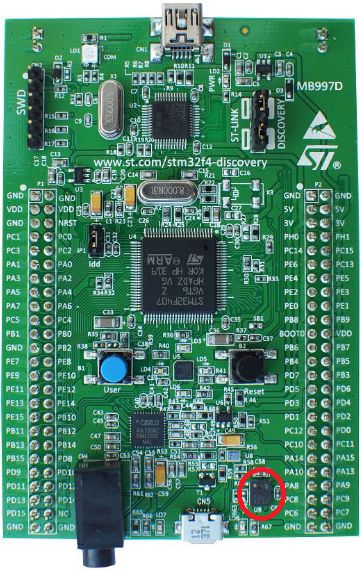
\includegraphics
	{files/images/board_view}
	\caption{View of the upper surface of the board, with the microphone highlighted in the circle.}
\end{figure}

In its bottom surface, it has 6 pins:
\begin{enumerate}
	\item \textbf{GND} - Connected to the GND of the board
	\item \textbf{LR} - Channel selection: used because the microphone is designed to allow stereo audio capture. If it is connected to GND, the MP45DT02 is placed in "left" channel mode: a sample is latched to the data output pin (PDM) on a falling edge of the clock, while on the rising clock edge, the output is set to high impedance. If the LR pin is connected to Vdd then the device operates in "right" channel mode and the MP45DT02 latches it's sample to PDM on a clock rising edge, setting the pin to high impedance on the falling edge of the clock.
	\item \textbf{GND} - Connected to the GND of the board
	\item \textbf{CLK} - Synchronization input clock: this pin is connected to the PB10 port of the board. The clock signal determines the sampling frequency.
	\item \textbf{DOUT} - PDM Data Output. Connected to the PC03 pin of the board's GPIO.
	\item \textbf{VDD} - Power supply.
\end{enumerate}

\begin{figure}[H]
	\centering
	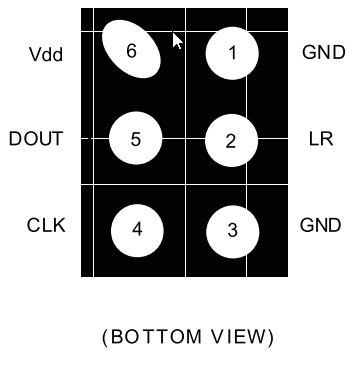
\includegraphics
	{files/images/mic_bottom_pins}
	\caption{Pins on the bottom of the microphone.}
\end{figure}

\subsection{Overview on sound acquisition and processing}
The sound is acquired by the microphone, and the communication with it happens through I2C.\\
The microphone acquires data in PDM format: each sample is a single bit, so the acquisition is a stream of bits; an high amplitude is represented with an high density of '1' bits in the bitstream. \\
The sampling frequency of the ADC is 11000 Hz. \\
In order to process the data, it has to be converted in PCM format: this is done by doing \textbf{CIC filtering}, with a decimation factor of 16 (each 16-bits sequence of 1-bit PDM samples is converted in one 16-bit PCM sample).\\
Then, an FFT analysis is performed on 4096 samples at a time to extract the fundamental frequency and the amplitude of the sound.

\subsection{Microphone initialization}
The initialization of the sound acquisition system comprehends several steps:
\begin{enumerate}
	\item SPI, DMA and General Purpose ports B and C are enabled through RCC
	\item GPIO ports are configured in \textit{Alternate} mode
	\item SPI is set to work in I2S mode
	\item interrupt handling for DMA is configured
	
\end{enumerate}

\subsection{Sound acquisition and processing}
Each time a new sample is ready:
\begin{enumerate}
	\item Read 16 bits from SPI and transfer them in RAM through DMA
	\item  Convert 16 PDM samples in one 16-bit PCM sample via \textbf{CIC filtering} with a decimation factor of 16
	\item Performs FFT through the \textit{arm\_cfft\_radix4\_f32}  module
	\item Calculates amplitude of each frequency with the \textit{arm\_cmplx\_mag\_f32} module
	\item calculates the Harmonic Product Spectrum to find the fundamental frequency (and its amplitude) in the vector
	\item Stores the values of the fundamental frequency and its amplitude in dedicated variables, then calls the \textbf{callback function} to react to the detected frequency.
\end{enumerate}